\chapter{Description of the problem setting for the course work}
\label{cha:Osnovania-ENG}


\section{Work Plan}

\begin{enumerate}
    \item Familiarize oneself with the literature.
    \item Formulate the goal and objectives of the work.
    \item Transition from a camera view to a top view (Projective Geometry).
    \item Solve the TSP problem for navigating players statically positioned on the field.
    \item Develop a simulation for debugging and testing the long-focus camera control algorithm.
    \begin{enumerate}
        \item Process pre-annotated data to build a heat map of player movement.
        \item Based on heat maps, implement a model of player movement on the field, closely matching their real-game movements.
        \item Develop simulations of camera projection onto the field (3D).
        \item Develop an API to control the camera in the simulation.
        \item Integrate object behavior simulation with camera simulation.
    \end{enumerate}
    \item Develop a metric that fairly evaluates the algorithm's performance.
    \item Develop a camera control algorithm with the best accuracy metrics.
    \begin{enumerate}
        \item Implement field traversal through points most visited by each player without predicting player movement (find the most frequent point for each player).
        \item Represent camera movement as a superposition of camera movement between zones and in a reference system tied to each zone.
        \item Implement player traversal considering predictions of player movement.
    \end{enumerate}
    \item Implement a PTZ camera model considering speed and acceleration constraints imposed on it. In the simplest case, neglect oscillations.
    \item Summarize the results.
\end{enumerate}

Assumptions:

1. The input data is well-labeled and accurately reflects the true locations of objects, with IDs not getting mixed up.

2. One camera has a view of the entire field, while the other is a telephoto camera.

3. If a face is turned within ±45 degrees towards the camera, it is considered possible to photograph (so positions of players are known at a given moment).

4. The height of the players is 170 cm, with the possibility of setting individual values.

5. If the face is captured within 150 pixels under the condition of point 3 and is not obstructed by other players, the player is photographed.

\section{Problem Statement}

Develop a mechanism for controlling a long-focus camera for efficient player detection and tracking within the field of view. A cyclic process is proposed, within which the camera automatically switches between players, adjusting the viewing angle and shooting distance. At the beginning of each iteration, the camera is focused on a new player, and the distance between them and the camera is optimized until the player's silhouette or face occupies a specified percentage of screen space - n\% (with a tolerance). After that, the camera remains fixed on the player for a certain number of frames k before moving to the next player for the next iteration of the process.

When using the term 'efficiently' in this context, it implies that the algorithm should perform optimally on various datasets, such as video recordings of football matches with player labels and their positions in each frame. An algorithm tested on a subset taken from the population of football matches should perform traversal with shooting in the shortest time possible.

\subsection{Coordinate Transformation}
A projectivity from one projective plane to another is called a plane-to-plane projectivity, though it is often simply referred to as a projectivity. It operates on and produces a homogeneous 3-vector, thus represented as a 3-by-3 matrix.

To understand how such a projectivity occurs, consider two images taken from different viewpoints of a plane within a scene, as illustrated in Figure 1. The mapping of points to their corresponding points in image 1 is defined by a projectivity. Similarly, the mapping of points to their corresponding points in image 2 is defined by another projectivity. An essential characteristic of projectivities is that they form a group. Consequently, there exists a projectivity that describes the mapping from the image of the plane in image 1 to the image of the plane in image 2 where.
$$ R = ST^{-1}$$

Given particular coordinates $X,\;Y$ a plane-to-plane projective transformation can be done as following:

$$
\begin{bmatrix}
\tau_{i}X' \\
\tau_{i}Y' \\
\tau_{i}
\end{bmatrix} = 
\underbrace{ \begin{bmatrix}
a_{1} & a_{2} & b_{1} \\
a_{3} & a_{4} & b_{2} \\
c_{1} & c_{2} & 1
\end{bmatrix} }_{ M } \begin{bmatrix}
X \\
Y \\
1
\end{bmatrix}
$$

Where $a_i$ are elements of a scaling/rotation matrix, $\begin{bmatrix}
    b_2 & b_1
\end{bmatrix}^T$ is a translation vector and $\begin{bmatrix}
    c_1 & c_2
\end{bmatrix}$ is a projection vector.

To find true new coordinates $X', Y'$ resulting vector has to be divided by $\tau_i$ that is the scaling factor. 

\subsubsection{Code implementation}

Given source image field corner coordinates in a list corner\_src\_points, a projective transformation matrix can be calculated. Function cv2.getPerspectiveTransform takes 2 arguments: source (4 coordinates (x,y), resembling corners of the input quadrilateral) and destination (4 coordinates (x,y), resembling corners of the output quadrilateral). On output the projective transformation matrix $M \in \mathbb{R}^{3 \times 3}$ described above is obtained.

\lstinputlisting[language=Python]{listings/projective_matrix.py}
\lstinputlisting[language=Python]{listings/coordinates_trans.py}
% add a link to library
Now by using this function and warpPerspective function from \textcolor{purple}{opencv} library, transformation can be done:
\begin{lstlisting}
corrected_image = cv2.warpPerspective(image, M, (width, height), borderValue=(255,255,255))
transform_coordinates(file_name="unscaled_track_df_new_coords.csv")
\end{lstlisting}

\section{Structure of the data}

Given a football field on which there are players and a ball, specified by coordinates $\vec X$, as functions of time $t$, in the reference system associated with the field. So we have an input array $X^{nm}_i$, where

$n$ - player number;

$m$ - describes one of the coordinates of the player’s position;

$i$ - describes a moment in time.

It is necessary to build a high-resolution camera axis control function (reserve $k$ for the camera number) with the given characteristics:

$F=(F_{min},F_{max})$ - focal length range;

$U=(u_1,u_2)$ - camera matrix size in pixels;

$p$ - matrix pixel size in meters (real world size of an image sensor's pixel);

$\Omega=(\omega_1, \omega_2)$ - maximum angular velocity in elevation and azimuth;

$\frac{dF}{dt}_{max}$ - maximum rate of change of focal length over time.

Camera coordinates in the reference system associated with the far left corner of the field

$$W=\{w_1,w_2,w_3\}$$

%Перенести в список терминов и определений

% \subsection{Фокусное расстояние (Focal Length)}
% Focal length is a distance between "nodal point" (that is where light converges in a lens) and a camera sensor\cite{FocalLength}. Cameras have a base focal length (max), but some cameras provide with a possibility to vary focal length by increasing/decreasing length of an objective (объектив). Thus a range of focal length ($F=(F_{min},F_{max})$) is of interest, as applications imply usages with long focus lenses.

%  \begin{figure}[!htbp]
%      \centering
%      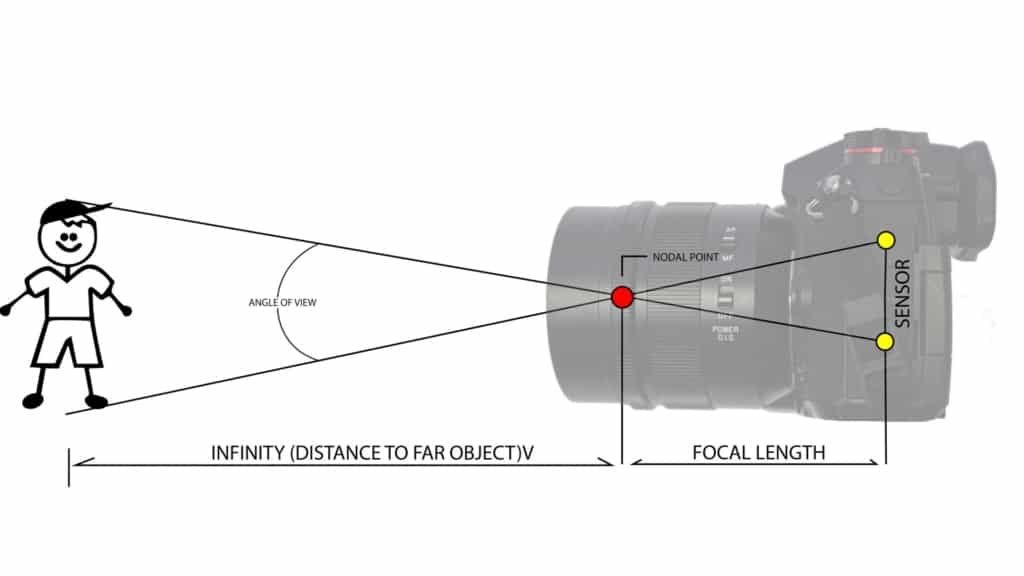
\includegraphics[width=0.8\linewidth]{figures/focal.jpg}
%      \caption{Focal Length}
%      \label{fig:enter-label}
%  \end{figure}

% \subsection{Матрица камеры (Image sensor)}
%  An image sensor refers to the electronic component in a digital camera that captures and converts light into digital signals, ultimately creating a digital image. The image sensor plays a crucial role in digital photography by replacing the traditional film used in film cameras. $U=(u_1,u_2)$ - sensor size of a camera in pixels represents number of pixels along $x$ and $y$ axes respectively, total image might have upmost $u_1*u_2$ pixels, given that photo is RGB, it can be calculated, that on an 3-dimensional tensor with shape $(u_1, u_2, 3)$ the whole image can be stored, and on 4-dimensional tensor with shape $(u_1, u_2, 3, \textbf{frames})$ a whole video may be stored frome such camera without audio-stream, where frames - is the amount of frames taken from that camera consequently.



% \subsection{Угловая Скорость (Angular Velocity)}
% An angular velocity is the speed of rotation for an object that can be stated as ${\displaystyle \omega ={\frac {d\varphi }{dt}}}$.

% \subsection{Угол Места; Элевация (Elevation)}
% Vertical angle of an observed object over true horizon. Elevation combined with azimuth are used for obtaining the direction to an object. \href{https://ru.wikipedia.org/wiki/%D0%A3%D0%B3%D0%BE%D0%BB_%D0%BC%D0%B5%D1%81%D1%82%D0%B0}{Elevation}

% \subsection{Азимут (Azimuth)}
% Horizontal angle evaluated from predefined direction (for example north) and direction of an observed object.

\section{The simplest task of controlling a high-resolution camera}

It is necessary to propose an algorithm for bypassing all players on the field, starting from the center of the field.

As a result we should get:

$\vec \psi(t)$ is a vector describing the elevation angle and azimuth of the camera sighting as a function of time.

At the same time, we must ensure that the player’s image is obtained in the camera’s field of view during the time $\Delta T$ corresponding to $R$ frames.

We consider the movement of the players to be a priori unknown.

1) The first step is to bypass stationary players

2) Second step - bypassing moving players

\subsection{Bypassing stationary players}

Given a weighted graph $G = (V, E)$, in our case complete, since from any vertex it can be rational to move to another, in the general case, where

$V$ - number of objects recognized in the frame, at this stage football players, $V = {1, 2, 3, ..., k}$

$E$ - edges of this graph;

$d_{ij}(i, j \in V, i \neq j)$ - the distance between two vertices $i, j$, and $d_{ij} > 0$, $d_{ij} \neq \infty$ and $d_{ij} = d_{ji}$.

We need to find a Hamiltonian cycle (closed path) such that
\begin{align}
     minD = \sum_{i,j \in V} d_{ij} * x_{ij},
\end{align}
Where
\begin{equation}
     x_{ij} =
     \begin{cases}
         1 & e_{ij} \in \text{optimal path}\\
         0 & e_{ij} \notin \text{optimal path}
     \end{cases}
\end{equation}
That is, $x_{ij}$ is a logical variable that turns to 1 if the edge $e_{ij}$ satisfies the condition of belonging to the optimal path, and 0 otherwise. The start and end of the round generally take place in the center of the football field. The result of the algorithm should be a path containing all the vertices of the graph and satisfying the conditions specified above.

\section{Approximations and limitations}
 
Moving the camera angle up/down left/right and focusing are independent of each other and can be done in parallel. (The metric being optimized depends on this)

 
We plan to have a different number of facilities and much greater than the number of football players. (The choice of algorithm depends on this - since the problem is NP hard, for a small amount it can be solved head-on - the 22 hypothesis is more optimal)

The camera should return to the starting point (center by default).

 
% It is impossible to assume that the running speed of a football player is negligible relative to the speed of the camera.
